\documentclass[12pt]{article}
\newif\ifblind
\blindfalse
% \blindtrue
% Common preamble of wellbeing.tex, wellbeing_region.tex and wellbeing_discrepancy.tex
% Compile from papers/:  latexmk -pdf -outdir=build <file>.tex
\usepackage[T1]{fontenc}
\usepackage[utf8]{inputenc}
\usepackage{lmodern}
\usepackage[margin=2.5cm]{geometry}
\usepackage{setspace}
\onehalfspacing
\usepackage{amsmath, amssymb}
\usepackage{graphicx}
\usepackage{booktabs, makecell, threeparttable, adjustbox}
\usepackage{caption}
\captionsetup{font=small, labelfont=bf}
\usepackage[authoryear, round]{natbib}
\bibliographystyle{apalike}
\usepackage{xspace}
\usepackage{xcolor}
\usepackage[colorlinks=true, linkcolor=blue!60!black, citecolor=blue!60!black, urlcolor=blue!60!black]{hyperref}
\usepackage{lineno}
% Placeholders for information to be completed by the author
\newcommand{\todo}[1]{\textcolor{red}{[TODO: #1]}}
% Numbers computed by code_wellbeing/main.R (percentages are given without the % sign)
\newcommand{\corGallupWHR}{0.993\xspace}
\newcommand{\corGallupWHRoldMapping}{0.89\xspace}
\newcommand{\nGallupCountryYears}{2351\xspace}
\newcommand{\nGallupCountries}{168\xspace}
\newcommand{\nWVSCountryYears}{304\xspace}
\newcommand{\nWVSCountries}{108\xspace}
\newcommand{\nWVSRespondents}{439531\xspace}
\newcommand{\nFabre}{11000\xspace}
\newcommand{\nFabreCountries}{10\xspace}
\newcommand{\bestIncome}{Cluster k=7 nominal\xspace}
\newcommand{\shareRegionBetterWVS}{86\xspace}
\newcommand{\shareRegionBetterWVSbest}{79\xspace}
\newcommand{\nSpecsWVS}{952\xspace}
\newcommand{\meanShareIncomeBest}{28\xspace}
\newcommand{\meanRtwoIncomeBest}{19\xspace}
\newcommand{\meanRtwoIncomePPP}{12\xspace}
\newcommand{\meanRtwoRegion}{37\xspace}
\newcommand{\RtwoSatisfiedMeanPPP}{20\xspace}
\newcommand{\RtwoHappinessMeanPPP}{4\xspace}
\newcommand{\RtwoVeryHappyPPP}{0\xspace}
\newcommand{\shareRegionBetterGallup}{35\xspace}
\newcommand{\shareIncomeGallupMean}{60\xspace}
\newcommand{\RtwoGallupMeanPPP}{61\xspace}
\newcommand{\RtwoGallupRegion}{48\xspace}
\newcommand{\RtwoWHRPPP}{63\xspace}
\newcommand{\RtwoWHRRegion}{55\xspace}
\newcommand{\shareRegionBetterNoLatamEE}{27\xspace}
\newcommand{\shareIncomeNoLatamEE}{34\xspace}
\newcommand{\shareRegionBetterContinents}{54\xspace}
\newcommand{\shareRegionBetterWB}{64\xspace}
\newcommand{\cvIncomeSatisfiedMean}{0.18\xspace}
\newcommand{\cvRegionSatisfiedMean}{0.44\xspace}
\newcommand{\cvIncomeGallupMean}{0.60\xspace}
\newcommand{\cvRegionGallupMean}{0.45\xspace}
\newcommand{\shareCvRegionBetterWVS}{100\xspace}
\newcommand{\corHappySatisfied}{0.72\xspace}
\newcommand{\corHappinessSatisfactionMean}{0.76\xspace}
\newcommand{\corVeryHappySatisfiedMean}{0.63\xspace}
\newcommand{\slopeVeryHappy}{0.005\xspace}
\newcommand{\pVeryHappy}{0.85\xspace}
\newcommand{\happiestFirst}{Switzerland\xspace}
\newcommand{\happiestFirstN}{10\xspace}
\newcommand{\happiestSecond}{Mexico\xspace}
\newcommand{\happiestSecondN}{9\xspace}
\newcommand{\happiestThird}{Kyrgyzstan\xspace}
\newcommand{\happiestThirdN}{6\xspace}
\newcommand{\happiestRegionWestern}{24\xspace}
\newcommand{\happiestRegionLatinAmerica}{19\xspace}
\newcommand{\happiestRegionAsia}{16\xspace}
\newcommand{\happiestRegionAfrica}{5\xspace}
\newcommand{\nHappiestCells}{64\xspace}
\newcommand{\treeRegionFirst}{8\xspace}
\newcommand{\withinRtwoSatisfiedMean}{0.22\xspace}
\newcommand{\withinSlopeSatisfiedMean}{1.68\xspace}
\newcommand{\crossSlopeSatisfiedMean}{1.09\xspace}
\newcommand{\withinSlopeVeryHappy}{0.18\xspace}
\newcommand{\pWithinVeryHappy}{0.004\xspace}
\newcommand{\nWithin}{272\xspace}
\newcommand{\RtwoFreedomSatisfaction}{63\xspace}
\newcommand{\shapleyFreedom}{40\xspace}
\newcommand{\shapleyFreedomRegion}{26\xspace}
\newcommand{\shapleyFreedomIncome}{9\xspace}
\newcommand{\RtwoTolerance}{21\xspace}
\newcommand{\RtwoGod}{0\xspace}
\newcommand{\RtwoGrowth}{2\xspace}
\newcommand{\nonresponseSatisfactionWVS}{1.5\xspace}
\newcommand{\nonresponseHappinessWVS}{1.7\xspace}
\newcommand{\corNonresponseGDP}{-0.08\xspace}
\newcommand{\effectLadder}{-0.45\xspace}
\newcommand{\seLadder}{0.05\xspace}
\newcommand{\effectScale}{0.14\xspace}
\newcommand{\seScale}{0.05\xspace}
\newcommand{\effectLadderZeroTen}{-0.46\xspace}
\newcommand{\effectScaleZeroTen}{-0.26\xspace}
\newcommand{\effectLadderSatisfied}{-9\xspace}
\newcommand{\interactionLadderIncome}{-0.004\xspace}
\newcommand{\pInteractionLadderIncome}{0.92\xspace}
\newcommand{\gradientIncomeSatisfaction}{0.69\xspace}
\newcommand{\pHeterogeneityWording}{0.000\xspace}
\newcommand{\chiHeterogeneityWording}{93.4\xspace}
\newcommand{\wordingCHE}{-0.34\xspace}
\newcommand{\wordingDEU}{-0.53\xspace}
\newcommand{\wordingESP}{-1.12\xspace}
\newcommand{\wordingFRA}{-0.50\xspace}
\newcommand{\wordingGBR}{-0.63\xspace}
\newcommand{\wordingITA}{-0.55\xspace}
\newcommand{\wordingJPN}{0.36\xspace}
\newcommand{\wordingPOL}{-0.55\xspace}
\newcommand{\wordingSAU}{-0.79\xspace}
\newcommand{\wordingUSA}{-0.63\xspace}
\newcommand{\wordingMin}{-1.12\xspace}
\newcommand{\wordingMax}{0.36\xspace}
\newcommand{\decompMeanGap}{-0.39\xspace}
\newcommand{\decompMeanQuestion}{-0.71\xspace}
\newcommand{\decompMeanResidual}{0.32\xspace}
\newcommand{\decompShareLevelQuestion}{1.83\xspace}
\newcommand{\decompVarShareQuestion}{-0.20\xspace}
\newcommand{\decompVarShareResidual}{1.20\xspace}
\newcommand{\decompMeanAbsGap}{0.43\xspace}
\newcommand{\decompMeanAbsResidual}{0.64\xspace}
\newcommand{\decompRmsePredictionGallup}{0.73\xspace}
\newcommand{\decompRmseNaive}{0.42\xspace}
\newcommand{\decompMeanGapSat}{-0.05\xspace}
\newcommand{\decompMeanQuestionSat}{-0.11\xspace}
\newcommand{\decompVarShareQuestionSat}{-0.11\xspace}
\newcommand{\decompSdGap}{0.44\xspace}
\newcommand{\decompSdQuestion}{0.45\xspace}
\newcommand{\decompSdResidual}{0.69\xspace}
\newcommand{\decompCorGapQuestion}{-0.20\xspace}
\newcommand{\decompLowMeanGap}{-0.44\xspace}
\newcommand{\decompHighMeanGap}{-0.34\xspace}
\newcommand{\decompLowMeanQuestion}{-0.85\xspace}
\newcommand{\decompHighMeanQuestion}{-0.56\xspace}
\newcommand{\decompLowMeanResidual}{0.17\xspace}
\newcommand{\decompHighMeanResidual}{0.46\xspace}
\newcommand{\decompLowVarShareQuestion}{-0.52\xspace}
\newcommand{\decompHighVarShareQuestion}{0.15\xspace}
\newcommand{\decompLowShareLevelQuestion}{1.42\xspace}
\newcommand{\decompHighShareLevelQuestion}{2.27\xspace}
\newcommand{\decompLowCorGapQuestion}{-0.47\xspace}
\newcommand{\decompHighCorGapQuestion}{0.14\xspace}
\newcommand{\nDecompCountries}{10\xspace}
\newcommand{\nSameYear}{7\xspace}
\newcommand{\nRecent}{4\xspace}
\newcommand{\varShareQuestionSameYear}{-0.27\xspace}
\newcommand{\varShareQuestionRecent}{-0.81\xspace}
\newcommand{\shareLevelQuestionSameYear}{1.60\xspace}
\newcommand{\shareLevelQuestionRecent}{1.19\xspace}
\newcommand{\meanSampleEffectGallup}{0.75\xspace}
\newcommand{\corFabreWHR}{0.75\xspace}
\newcommand{\minSampleEffectGallup}{0.16\xspace}
\newcommand{\maxSampleEffectGallup}{1.24\xspace}
\newcommand{\meanSampleEffectWVS}{0.54\xspace}
\newcommand{\meanFabreGallupZero}{5.93\xspace}
\newcommand{\meanFabreWVSOne}{6.64\xspace}
\newcommand{\sampleEffectUSWVS}{0.49\xspace}
\newcommand{\nCommon}{149\xspace}
\newcommand{\nCommonCountries}{83\xspace}
\newcommand{\RtwoCommonGallup}{0.49\xspace}
\newcommand{\RtwoCommonWVS}{0.11\xspace}
\newcommand{\slopeCommonGallup}{1.76\xspace}
\newcommand{\slopeCommonWVS}{0.77\xspace}
\newcommand{\slopeGapGDP}{1.07\xspace}
\newcommand{\seSlopeGapGDP}{0.16\xspace}
\newcommand{\RtwoGapGDP}{0.31\xspace}
\newcommand{\slopeQuestionGDP}{0.30\xspace}
\newcommand{\seSlopeQuestionGDP}{1.75\xspace}
\newcommand{\RtwoAdjustedWVS}{0.20\xspace}
\newcommand{\shareIncomeCommonGallup}{51\xspace}
\newcommand{\shareIncomeCommonWVS}{15\xspace}

\newcommand{\Rsq}{\ensuremath{R^2}\xspace}
% Switch: show region-specific material (set to false in wellbeing_discrepancy.tex)
\newif\ifshowregion
\showregiontrue

% Split paper 1: predictive capacity of GDP per capita vs. world region for national well-being (max. 9,000 words excluding appendices).
% Compile from papers/:  latexmk -pdf -outdir=build wellbeing_region.tex

\title{Is GDP per Capita a Good Predictor of National Well-Being?\\ Income versus World Regions\thanks{Data and code: \url{https://github.com/bixiou/wellbeing_gdp_region} \todo{public repository (e.g.\ OSF); Gallup data cannot be redistributed}. I thank Claudia Senik and participants in the 2024 STATEC Well-being Conference for helpful comments, Armon Rezai and the Vienna University of Economics and Business (WU Wien) for access to the Gallup World Poll data, and Julieta Toffoli for research assistance. This research did not receive any specific grant from funding agencies in the public, commercial, or not-for-profit sectors. Declaration of interest: none.}}
\author{Adrien Fabre\\ \small CNRS, CIRED \todo{postal address}\\ \small \href{mailto:adrien.fabre@cnrs.fr}{adrien.fabre@cnrs.fr}}
\date{\today}

\begin{document}
\maketitle

\begin{abstract}
\noindent Across countries, national well-being is commonly described as an increasing function of log GDP per capita. I assess how much of national well-being GDP per capita actually predicts, and benchmark it against a simple alternative: the country's world region. Using all waves of the World Values Survey and the European Values Study (1981--2023, \nWVSCountries countries), eight well-being indicators and seven income measures, I find that log GDP per capita explains on average \meanRtwoIncomePPP\% of the cross-country variance of well-being, and nothing of the share of very happy people. Region is a better predictor in \shareRegionBetterWVS\% of \nSpecsWVS specifications and, out of sample, for every indicator. This advantage is driven by Latin America (happier than its income predicts) and Eastern Europe (unhappier), and it does not hold in the Gallup World Poll, where income predicts life evaluations as well as region. Within countries, however, well-being rises with GDP over time. Whether GDP is a poor predictor of national well-being thus depends on the data and on a few large regional deviations.
\end{abstract}

\noindent\textbf{Keywords:} subjective well-being; life satisfaction; happiness; GDP; world regions; Easterlin paradox.\\
\noindent\textbf{JEL codes:} I31; O15; O57.

% \linenumbers
\section{Introduction}\label{sec:intro}

Which country is the happiest? The answer most often heard, based on the World Happiness Report, is a Scandinavian, high-income country. Behind this answer lies one of the most cited stylized facts of well-being research: across countries, average life evaluations increase with the logarithm of GDP per capita \citep{deaton_income_2008,stevenson_economic_2008,sacks_new_2012}. Using the Gallup World Poll, \citet{deaton_income_2008} finds a correlation above 0.8 between average life evaluation and log GDP per capita; using the World Values Survey (WVS), \citet{inglehart_genes_2000} reported an $R^2$ of about one half for an index combining happiness and life satisfaction. These correlations are frequently invoked to support the view that economic growth is a reliable route to well-being.

This paper asks how much of national well-being GDP per capita actually predicts, and whether it predicts it better than a very simple alternative, the country's world region. Region is a natural benchmark: previous work has documented that Latin American countries report higher well-being than their income would predict \citep{graham_paradox_2009,rojas_handbook_2016,inglehart_development_2008} and former communist countries lower well-being \citep{guriev_unhappiness_2009}, and that cultural factors shape national well-being \citep{diener_culture_2000,diener_personality_2003,exton_comparing_2015,senik_french_2014}. But the relative predictive power of income and region has not, to my knowledge, been systematically compared.

I use all seven waves of the WVS, complemented with the 2017 wave of the European Values Study (\nWVSCountryYears country-years), eight indicators of national well-being based on the happiness and life-satisfaction questions, and seven income measures (log GDP per capita at PPP or market exchange rates, income sextiles, and income clusters). Since the ranking of groups can depend on the choice of indicator \citep{bond_sad_2019}, I consider all of them. I compare the variance explained by income and by region using the Shapley (LMG) decomposition of $R^2$ \citep{lindeman_introduction_1980,gromping_estimators_2007}, adjusted $R^2$, and leave-one-country-out cross-validation, which directly measures predictive capacity. I then examine the robustness of the results across waves, samples, classifications of regions, and datasets, using the Gallup World Poll and the World Happiness Report.

Four findings emerge. First, in the WVS, GDP per capita is a weak predictor of national well-being: log GDP per capita explains on average \meanRtwoIncomePPP\% of the variance of the eight indicators, and nothing of the share of very happy people. Second, region is a better predictor than income in \shareRegionBetterWVS\% of specifications and, out of sample, for every indicator. Third, this conclusion must be qualified: the advantage of region is driven by Latin America and Eastern Europe, it weakens with classifications that do not isolate these two groups, and it does not hold in Gallup, where log GDP explains \RtwoGallupMeanPPP\% of the variance of the mean ladder against \RtwoGallupRegion\% for region. Fourth, within countries, well-being increases with GDP over time.

The paper contributes to the literature on income and well-being across countries \citep{easterlin_does_1974,easterlin_happiness_2010,stevenson_economic_2008,deaton_income_2008,jebb_happiness_2018} by quantifying the predictive capacity of income out of sample, benchmarking it against regions, and showing that the strength of the cross-country relationship depends on the dataset. A companion paper \todo{cite companion paper} uses a survey experiment to show that question wording accounts for about half of the difference in predictive capacity between Gallup and the WVS, but not for their different income gradients.

Section~\ref{sec:data} presents the data, Section~\ref{sec:results} the results, Section~\ref{sec:discussion} discusses them, and Section~\ref{sec:conclusion} concludes.

\section{Data}\label{sec:data}
% Shared section: data on national well-being, income and regions (WVS, Gallup, WHR, WDI)
\subsection{World Values Survey}\label{subsec:wvs}

The World Values Survey (WVS) is the longest-running cross-national survey of values and subjective well-being. I use the WVS time-series file \citep{wvs_trend_2022}, which pools the seven waves conducted between 1981 and 2022, and complete it with the Joint EVS/WVS 2017--2022 dataset \citep{evs_wvs_joint_2024}, which adds the \nEVSSurveys national surveys of the 2017 wave of the European Values Study (EVS, conducted in 2017--2021) and \nNewWVSSurveys recent WVS surveys (India 2023, Uzbekistan 2022). The EVS asks the same well-being questions, and the combination of the two surveys is standard practice (the so-called Integrated Values Surveys). The EVS and the WVS are distinct surveys: when both surveyed the same country the same year (\nEVSSameYearWVS cases), I keep both surveys as separate observations.
For brevity, I refer to the combined data as the WVS: \nWVSRespondents respondents in \nWVSCountryYears country-years and \nWVSCountries countries. National samples are designed to be representative of the adult population, typically with 1,000 to 3,000 respondents, and most interviews are conducted face-to-face (though some recent national surveys used web, mail or mixed modes, e.g.\ the WVS in the United States in 2017 and in Japan in 2019, or the EVS in Switzerland in 2017). All statistics use the survey weights provided by the WVS and the EVS.

The WVS contains two questions on subjective well-being:
\begin{itemize}
    \item \textit{Happiness}: ``Taking all things together, would you say you are: \textit{Very happy}; \textit{Quite happy}; \textit{Not very happy}; \textit{Not at all happy}.''
    \item \textit{Life satisfaction}: ``All things considered, how satisfied are you with your life as a whole these days?'', answered on a scale from 1 (\textit{Completely dissatisfied}) to 10 (\textit{Completely satisfied}).
\end{itemize}
Non-responses are rare (\nonresponseSatisfactionWVS\% for satisfaction and \nonresponseHappinessWVS\% for happiness on average) and uncorrelated with GDP per capita (correlation: \corNonresponseGDP); they are excluded.

\ifshowregion
\paragraph{Indicators of national well-being.}
Because there is no consensus on how to aggregate ordinal answers into a national indicator, and because the ranking of countries can depend on this choice \citep{bond_sad_2019}, I compute eight indicators for each country-year:
\begin{itemize}
    \item \textit{Happy}: share answering \textit{Quite} or \textit{Very happy};
    \item \textit{Very Happy}: share answering \textit{Very happy};
    \item \textit{Very Unhappy}: share answering \textit{Not at all happy};
    \item \textit{V.~Happy -- V.~Unhappy}: difference between the two previous shares;
    \item \textit{Happiness (mean)}: mean happiness, with answers coded $+3$, $+1$, $-1$, $-3$;
    \item \textit{Satisfaction (mean)}: mean life satisfaction;
    \item \textit{Satisfied}: share answering 6 to 10 to the life-satisfaction question;
    \item \textit{Happy + Satisfied}: average of \textit{Happy} and \textit{Satisfied}, the index used by \citet{inglehart_genes_2000}.
\end{itemize}
The indicators are positively but imperfectly correlated: across country-years, the correlation between \textit{Happy} and \textit{Satisfied} is \corHappySatisfied, and between \textit{Very Happy} and \textit{Satisfaction (mean)} it is only \corVeryHappySatisfiedMean (Appendix Table~\ref{tab:correlation}).
\fi

\subsection{Gallup World Poll and World Happiness Report}\label{subsec:gallup}

The Gallup World Poll interviews around 1,000 adults per country and year in more than 140 countries, by telephone where coverage is high (typically in high-income countries) and face-to-face elsewhere \citep{gallup_methodology_2022}. Its life-evaluation question is the Cantril ladder \citep{cantril_pattern_1965}: ``Please imagine a ladder, with steps numbered from 0 at the bottom to 10 at the top. The top of the ladder represents the best possible life for you and the bottom of the ladder represents the worst possible life for you. On which step of the ladder would you say you personally feel you stand at this time?''

I use the distribution of answers by country and wave, tabulated from the Gallup World Poll microdata (\nGallupCountryYears country-years, \nGallupCountries countries, 2006--2023), from which I compute the mean and the shares answering 6--10, 8--10, 9--10, 10, 0--4 and 0--2. These distributions are unweighted. To cover the most recent years, I also use the ladder means published in the World Happiness Report 2026 \citep{whr_2026}, which average Gallup data over three years up to 2023--2025.

\subsection{Income}\label{subsec:income}

My benchmark income measure is the log of GDP per capita at purchasing power parity (PPP, constant 2021 international dollars) from the World Development Indicators \citep{worldbank_wdi_2026}. As an alternative, I use GDP per capita at market exchange rates (constant 2015 US dollars). Missing values are filled in automatically, in three steps: (i) PPP series, which start in 1990, are extended backwards (and gaps filled) using the growth rate of real GDP per capita; (ii) for countries absent from the World Bank data (e.g. Taiwan, or Venezuela in recent years), I use the IMF World Economic Outlook \citep{imf_weo_2026}, converted into the constant dollars of the World Bank series with a U.S. price deflator (the ratio of World Bank to IMF values for the United States); (iii) remaining gaps are filled with the closest year available (Montenegro 1996). Territories without national accounts use the GDP of the closest entity (e.g. the United Kingdom for Northern Ireland). A robustness check excludes all imputed values.

\ifshowregion
Region is a categorical variable, which can capture non-linear patterns that a single continuous variable cannot. To compare income and region on an equal footing, I also use categorical income indicators: income sextiles and income clusters obtained by $k$-means clustering of log GDP per capita, with $k = 5$, 6 or 7, recomputed in each estimation sample. The clusters let the data choose the thresholds between income groups and allow for non-linear relationships.
\fi

\ifshowregion
\subsection{Regions}\label{subsec:regions}

My main classification groups countries into the five UN regional groups (Figure~\ref{fig:regions}): \textit{Africa}, \textit{Asia} (the Asia-Pacific group, which includes the Middle East and Central Asia), \textit{Eastern Europe} (the former Eastern Bloc, excluding Central Asia), \textit{Latin America} (including the Caribbean), and \textit{Western} countries (the ``Western European and Others'' group: Western Europe, North America, Australia, New Zealand, and Turkey). It departs from the UN groups for two countries only: Israel, a member of the Western group since 2000 because it was denied access to the Asia-Pacific group, is classified in Asia, and Cyprus, a member of the Asia-Pacific group, is classified with Western countries. Territories that are not UN members (e.g.\ Taiwan, Hong Kong, Puerto Rico, Kosovo) are assigned to the group of their neighbors.
For robustness, I use four alternative classifications: the exact UN regional groups (with Israel in the Western group and Cyprus in Asia); a six-region variant separating the Middle East and grouping Central Asia with Eastern Europe; the seven World Bank regions (East Asia and Pacific, Europe and Central Asia, Latin America and the Caribbean, Middle East and North Africa, North America, South Asia, Sub-Saharan Africa), which isolate Latin America but group Eastern and Western Europe; and the five continents (Africa, Americas, Asia, Europe, Oceania), which isolate neither Latin America nor Eastern Europe.

\begin{figure}[htbp]
    \centering
    \caption{Main classification of countries into five world regions.}\label{fig:regions}
    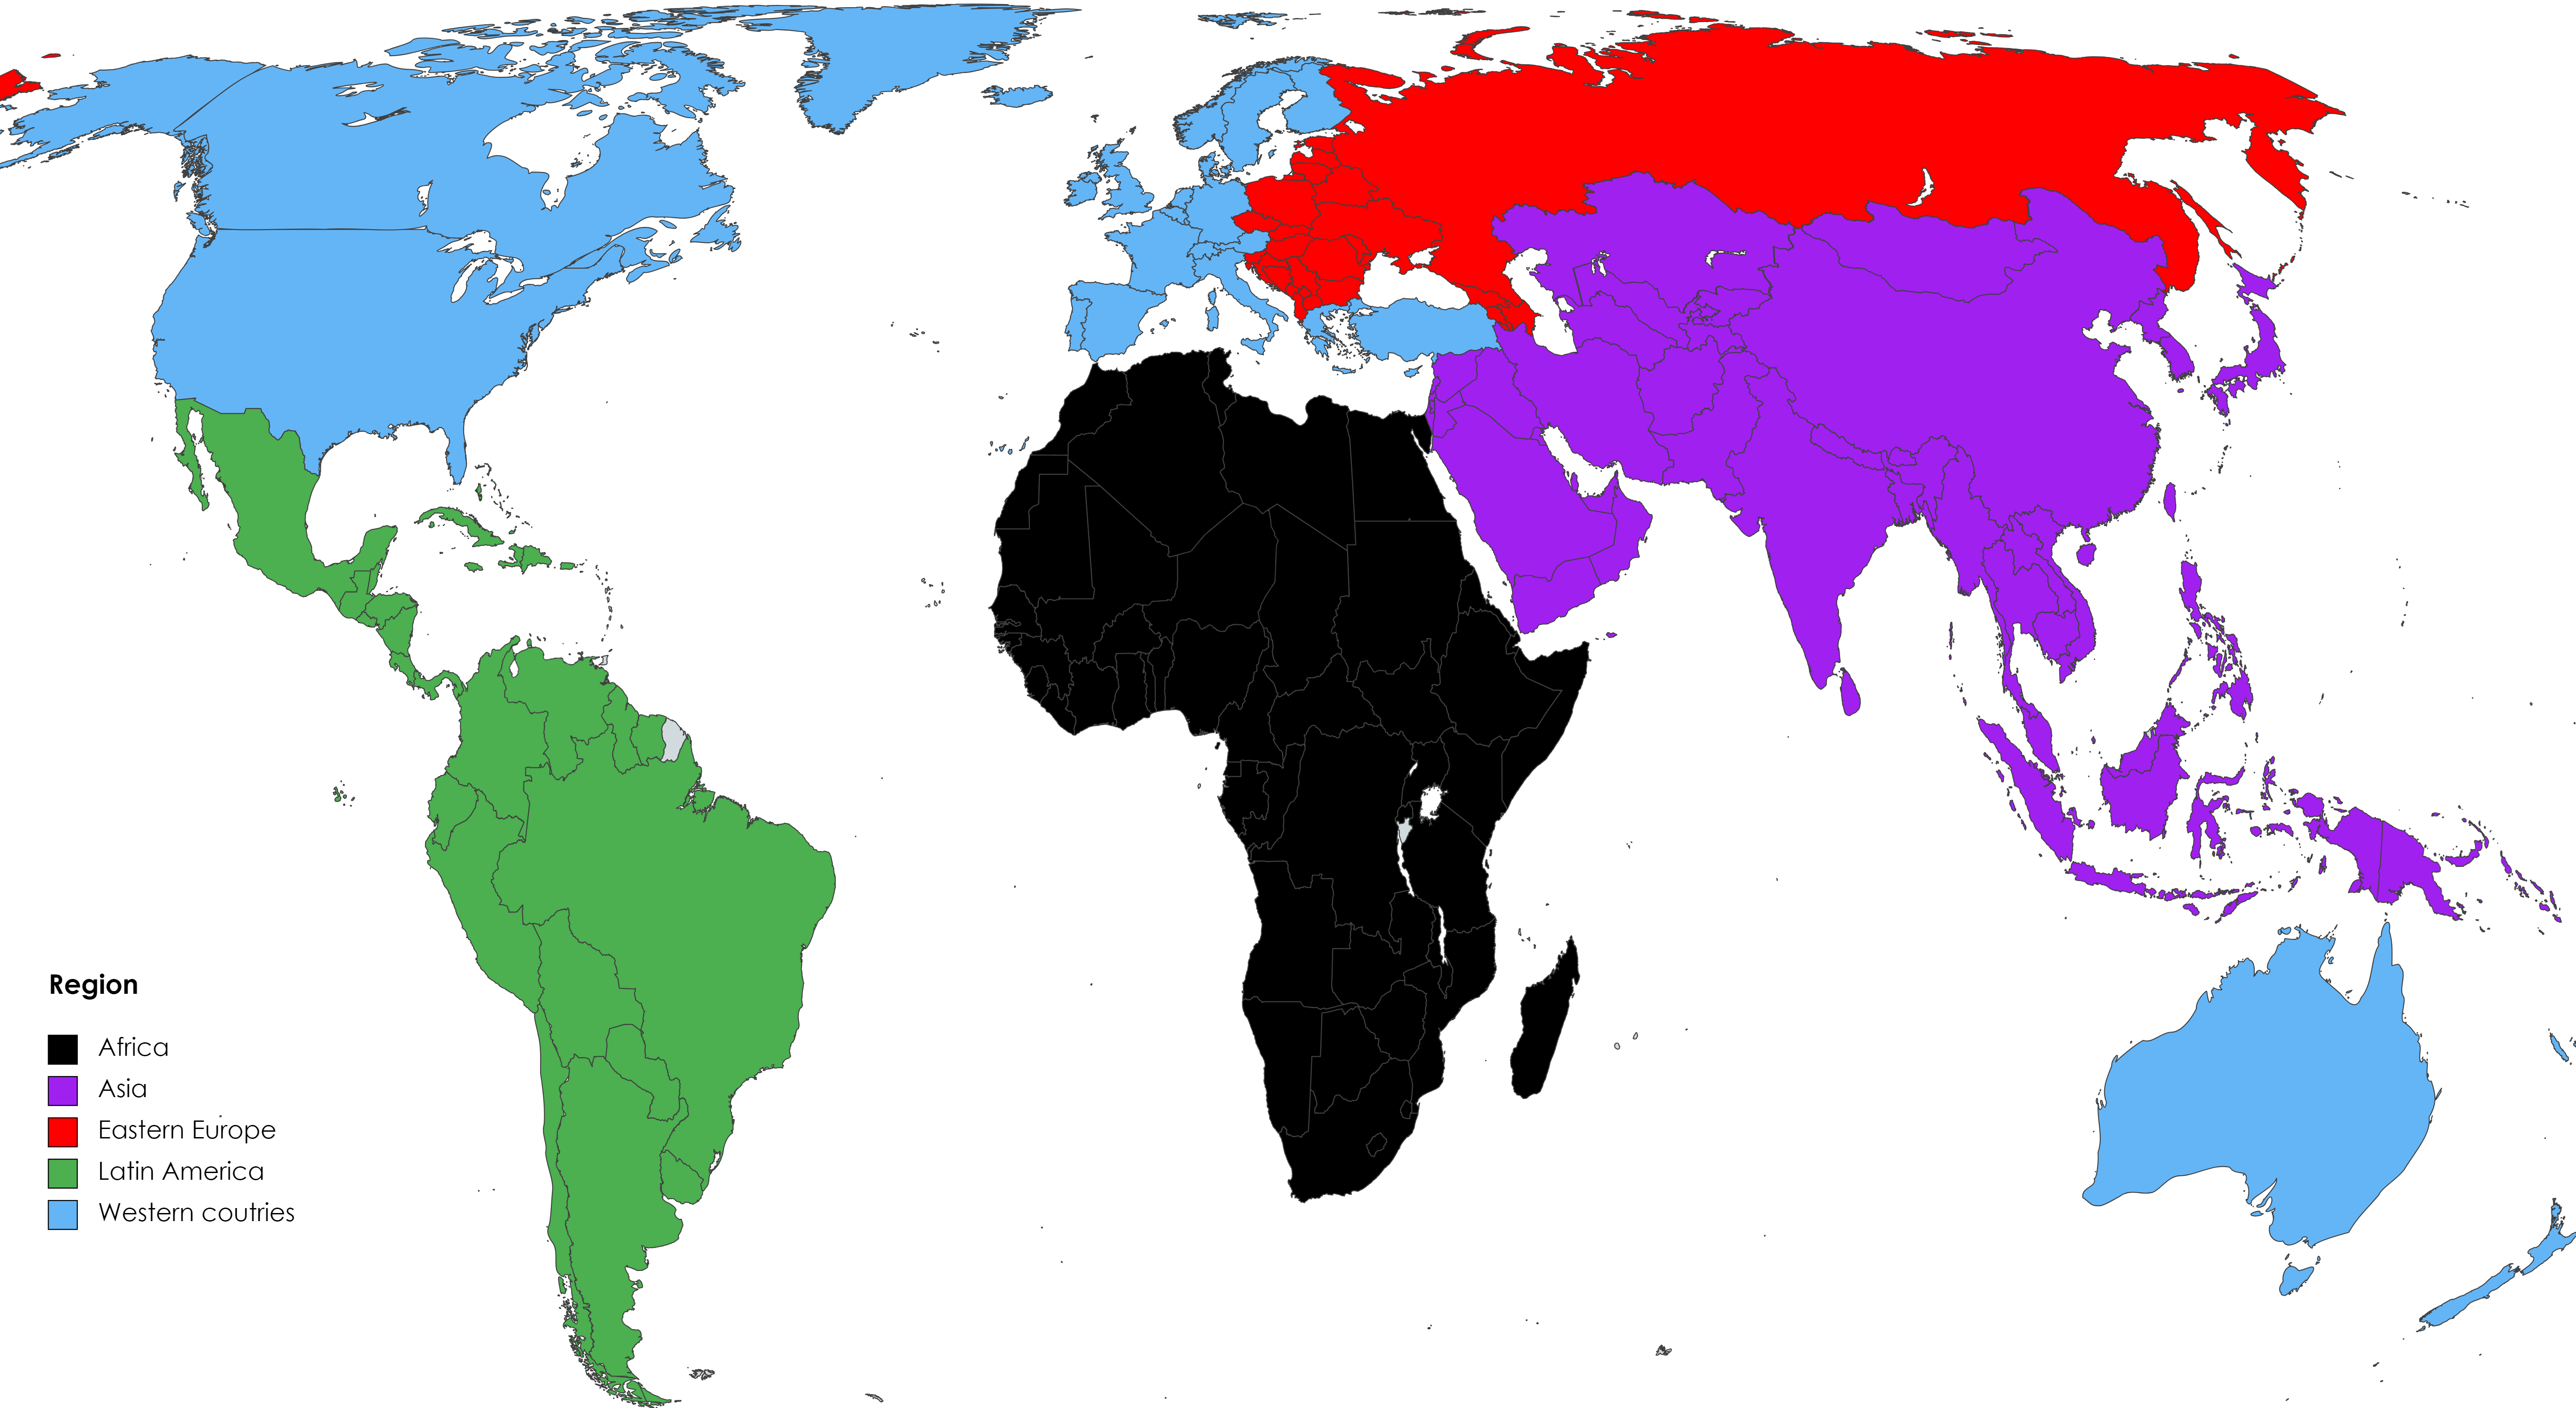
\includegraphics[width=.9\textwidth]{../figures/region_groupings.png}
\end{figure}
\fi

\section{Results}\label{sec:results}
% Shared section: income, region and national well-being (method and results)
\subsection{Empirical strategy}\label{subsec:method_region}

For each well-being indicator and each income indicator, I estimate three linear regressions across country-years $i$:
\begin{align}
    well\text{-}being_i &= \alpha_1 + \beta_1\, income_i + u_i \label{eq:income}\\
    well\text{-}being_i &= \alpha_2 + \gamma_2\, region_i + e_i \label{eq:region}\\
    well\text{-}being_i &= \alpha_3 + \beta_3\, income_i + \gamma_3\, region_i + \varepsilon_i \label{eq:both}
\end{align}
where $region_i$ denotes the vector of region dummies. Denoting $R^2_1$, $R^2_2$ and $R^2_3$ their coefficients of determination, the share of the variance explained by income alone is $R^2_1$. To compare income and region, I decompose $R^2_3$ between the two regressors following \citet{lindeman_introduction_1980} (LMG), i.e.\ using the Shapley value \citep{gromping_estimators_2007}. With two (groups of) regressors, the LMG contribution of income is the average of its contribution when entered first ($R^2_1$) and when entered second ($R^2_3 - R^2_2$). The \textit{share of explained variance due to income} is therefore
\begin{equation}
    s = \frac{R^2_1 + (R^2_3 - R^2_2)}{2\, R^2_3}, \label{eq:share}
\end{equation}
and region is the better predictor whenever $s < 50\%$.

One feature of this comparison could favor region: region has four degrees of freedom while log GDP has one. I address this concern in three ways. First, I use categorical income variables (sextiles and clusters) with as many or more categories as regions. Second, I compute $s$ with adjusted $R^2$, which penalizes additional regressors; with more than 300 observations, the adjustment is small and only reinforces the conclusions. Third, and more directly relevant to \textit{predictive} capacity, I compute leave-one-country-out cross-validated $R^2$: each country's observations are predicted by a model estimated on all other countries. Unlike the in-sample $R^2$, the cross-validated $R^2$ decreases when a model has superfluous parameters, and it is negative when a model predicts worse than the sample mean. Other robustness checks include each WVS wave separately, excluding the EVS surveys, weighting countries by their population, keeping only the last observation of each country, excluding the pandemic years 2020--2021, excluding imputed GDP values, using the previous vintage of GDP data (PPP in constant 2017 dollars), alternative region classifications, and excluding Latin America or Eastern Europe.

\subsection{Income explains a small share of national well-being in the WVS}\label{subsec:r2_income}

Figure~\ref{fig:satisfaction_gdp} plots mean life satisfaction against GDP per capita for all WVS country-years. The relationship is positive, but the dispersion at any given income level is large: countries with a GDP per capita around 10,000 dollars span most of the range of observed life satisfaction, from the former Soviet republics at the bottom to Latin American countries at the top. Log GDP per capita explains \RtwoSatisfiedMeanPPP\% of the variance of mean satisfaction. The relation is even weaker for happiness (Figure~\ref{fig:happiness_mean_gdp}). Appendix Figures~\ref{fig:very_happy_gdp}--\ref{fig:happy_gdp_w7_weighted} plot the other indicators.

\begin{figure}[htbp]
    \centering
    \caption{Mean life satisfaction vs.\ GDP per capita (PPP), WVS/EVS 1981--2023.}\label{fig:satisfaction_gdp}
    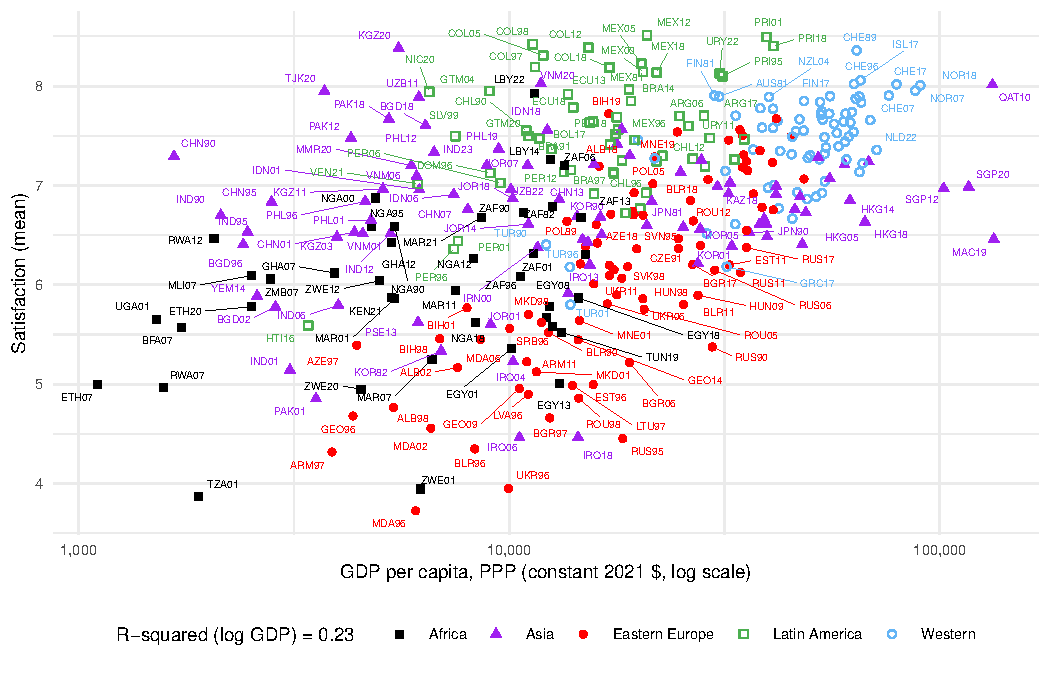
\includegraphics[width=.95\textwidth]{../figures/main/wvs_satisfied_mean_vs_gdp_ppp.pdf}
\end{figure}

\begin{figure}[htbp]
    \centering
    \caption{Mean happiness vs.\ GDP per capita (PPP), WVS/EVS 1981--2023.}\label{fig:happiness_mean_gdp}
    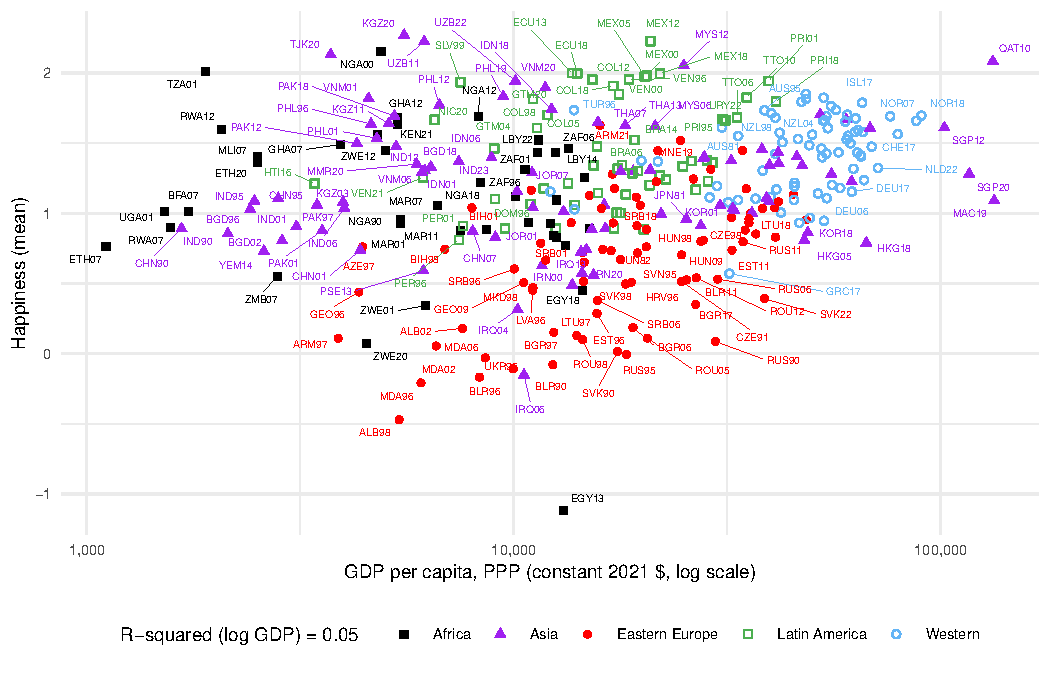
\includegraphics[width=.95\textwidth]{../figures/main/wvs_happiness_mean_vs_gdp_ppp.pdf}
    \begin{minipage}{.95\textwidth}\footnotesize \textit{Note:} Answers coded $+3$ (\textit{Very happy}), $+1$, $-1$, $-3$ (\textit{Not at all happy}).\end{minipage}
\end{figure}

Table~\ref{tab:r2_income} generalizes this result to all indicators and income measures. On average over the eight indicators, log GDP per capita at PPP explains \meanRtwoIncomePPP\% of the variance, and the best-performing income measure (\bestIncome) explains \meanRtwoIncomeBest\%. Satisfaction-based indicators are better explained than happiness-based ones: log GDP explains \RtwoHappinessMeanPPP\% of the variance of mean happiness and essentially none of the share of \textit{Very happy} people, whose slope with respect to log GDP is statistically indistinguishable from zero (slope \slopeVeryHappy, $p \pVeryHappy$; Appendix Table~\ref{tab:slopes}). This confirms the observation of \citet{deaton_income_2008} and \citet{inglehart_development_2008} that income is more closely related to life evaluation than to happiness. By contrast, region alone explains \meanRtwoRegion\% of the variance on average, and scores high even on happiness-based variables (last column).

\begin{table}[htbp]
    \centering
    \caption{Share of the variance of national well-being explained by income alone ($R^2$), WVS/EVS 1981--2023.}\label{tab:r2_income}
    \begin{adjustbox}{max width=\textwidth}
    \begin{tabular}{lcccccccc}
\toprule
Well-being indicator & \multicolumn{2}{c}{log GDP p.c.} & Sextile & \multicolumn{4}{c}{Income cluster} \\ & PPP & nominal & PPP & $k$=5 PPP & $k$=6 PPP & $k$=7 PPP & $k$=7 nominal & Region \\
\midrule
Happy & 0.13 & 0.18 & 0.20 & 0.19 & 0.19 & 0.20 & 0.23 & 0.36 \\
Very Happy & 0.00 & 0.00 & 0.03 & 0.02 & 0.03 & 0.04 & 0.03 & 0.35 \\
Very Unhappy & 0.06 & 0.09 & 0.12 & 0.11 & 0.13 & 0.13 & 0.14 & 0.16 \\
V. Happy -- V. Unhappy & 0.00 & 0.01 & 0.05 & 0.03 & 0.04 & 0.05 & 0.04 & 0.36 \\
Happiness (mean) & 0.04 & 0.07 & 0.10 & 0.08 & 0.09 & 0.10 & 0.10 & 0.38 \\
Satisfaction (mean) & 0.20 & 0.26 & 0.21 & 0.19 & 0.19 & 0.21 & 0.26 & 0.48 \\
Satisfied & 0.28 & 0.35 & 0.30 & 0.28 & 0.28 & 0.30 & 0.35 & 0.45 \\
Happy + Satisfied & 0.25 & 0.32 & 0.28 & 0.27 & 0.27 & 0.29 & 0.33 & 0.46 \\
\midrule
Mean & 0.12 & 0.16 & 0.16 & 0.15 & 0.15 & 0.17 & 0.19 & 0.37 \\
Max & 0.28 & 0.35 & 0.30 & 0.28 & 0.28 & 0.30 & 0.35 & 0.48 \\
\bottomrule
\end{tabular}

    \end{adjustbox}
    \begin{minipage}{\textwidth}\footnotesize \textit{Note:} $R^2$ of the regression of each well-being indicator (rows) on each income indicator (columns), over \nWVSCountryYears WVS/EVS country-years (a few with missing GDP are excluded). The last column gives the $R^2$ of the regression on region dummies. The replication files include an Excel version of this table with the $R^2$ of all region classifications (\texttt{tables/main/r2\_income\_all\_regions.xlsx}).\end{minipage}
\end{table}

\subsection{Region predicts national well-being better than income in the WVS}\label{subsec:region_wvs}

Table~\ref{tab:share_income} reports the share of explained variance due to income, $s$, for each indicator and income measure. It is below 50\% in all cases but one, where income and region are tied (0.50). On average, the best income measure accounts for \meanShareIncomeBest\% of the variance explained jointly by income and region. The first split of a regression tree using log GDP and region as candidate variables is on region for all national well-being indicators.

\begin{table}[htbp]
    \centering
    \caption{Share of explained variance due to income rather than region (LMG), WVS/EVS 1981--2023.}\label{tab:share_income}
    \begin{adjustbox}{max width=\textwidth}
    \begin{tabular}{lccccccc}
\toprule
Well-being indicator & \multicolumn{2}{c}{log GDP p.c.} & Sextile & \multicolumn{4}{c}{Income cluster} \\ & PPP & nominal & PPP & $k$=5 PPP & $k$=6 PPP & $k$=7 PPP & $k$=7 nominal \\
\midrule
Happy & 0.22 & 0.29 & 0.31 & 0.30 & 0.30 & 0.32 & 0.34 \\
Very Happy & 0.00 & 0.01 & 0.07 & 0.05 & 0.08 & 0.10 & 0.07 \\
Very Unhappy & 0.22 & 0.31 & 0.41 & 0.38 & 0.43 & 0.44 & 0.45 \\
V. Happy -- V. Unhappy & 0.01 & 0.02 & 0.09 & 0.06 & 0.09 & 0.11 & 0.08 \\
Happiness (mean) & 0.07 & 0.11 & 0.15 & 0.13 & 0.15 & 0.16 & 0.15 \\
Satisfaction (mean) & 0.25 & 0.30 & 0.25 & 0.23 & 0.23 & 0.25 & 0.30 \\
Satisfied & 0.35 & 0.41 & 0.36 & 0.34 & 0.35 & 0.37 & 0.41 \\
Happy + Satisfied & 0.31 & 0.38 & 0.35 & 0.33 & 0.34 & 0.35 & 0.39 \\
\midrule
Mean & 0.18 & 0.23 & 0.25 & 0.23 & 0.25 & 0.26 & 0.28 \\
Max & 0.35 & 0.41 & 0.41 & 0.38 & 0.43 & 0.44 & 0.45 \\
\bottomrule
\end{tabular}

    \end{adjustbox}
    \begin{minipage}{\textwidth}\footnotesize \textit{Note:} Share of the $R^2$ of Equation~\eqref{eq:both} attributed to income by the LMG (Shapley) decomposition, Equation~\eqref{eq:share}. Values below 0.5 indicate that region is the better predictor. Values above 0.5 (income is the better predictor) are in bold.\end{minipage}
\end{table}

The result is not an artifact of the larger number of parameters of the region model. Out of sample, region predicts better than income for every indicator (Appendix Table~\ref{tab:cv}): for mean satisfaction, the leave-one-country-out $R^2$ is \cvRegionSatisfiedMean with region against \cvIncomeSatisfiedMean with log GDP, and for several happiness indicators, income has no out-of-sample predictive power at all (negative cross-validated $R^2$). Across the \nSpecsWVS estimates of the robustness checks (indicator $\times$ income measure $\times$ specification; Appendix Table~\ref{tab:robustness}), region is the better predictor in \shareRegionBetterWVS\% of cases (\shareRegionBetterWVSbest\% with the best income measure). The result holds in each wave except wave 4 (1999--2004, 40 countries), where income and region perform similarly; when countries are weighted by population; without the EVS surveys; without the pandemic years; without imputed GDP values; and with the previous vintage of GDP data.

\subsection{Where the region advantage comes from}\label{subsec:region_limits}

Table~\ref{tab:region_classifications} shows that the region advantage rests on two well-known ``anomalies'': Latin America, happier than its income would predict \citep{graham_paradox_2009,rojas_handbook_2016}, and Eastern Europe, unhappier \citep{guriev_unhappiness_2009}. Region remains the better predictor when either one is excluded (in \shareRegionBetterNoLatam\% of cases without Latin America and \shareRegionBetterNoEE\% without Eastern Europe), but not when both are (\shareRegionBetterNoLatamEE\%). Consistently, the result holds with classifications that isolate both groups (exact UN groups and six regions: \shareRegionBetterUN\%), weakens with the World Bank regions, which isolate Latin America but merge Eastern and Western Europe (\shareRegionBetterWB\%), and disappears with continents, which isolate neither (\shareRegionBetterContinents\%).

\begin{table}[htbp]
    \centering
    \caption{Income vs.\ region by region classification and without Latin America or Eastern Europe (WVS/EVS).}\label{tab:region_classifications}
    \begin{adjustbox}{max width=\textwidth}
    \begin{tabular}{lcccccc}
\toprule
Region classification & Groups & Obs. & $R^2$ income & $R^2$ region & Share due to income & Region better \\ & & & (log PPP) & & (log PPP) & (share of cases) \\
\midrule
5 UN regional groups (main) & 5 & 340 & 0.14 & 0.33 & 0.23 & \textbf{0.98} \\
Exact UN regional groups & 5 & 340 & 0.14 & 0.33 & 0.23 & \textbf{1.00} \\
6 regions (Middle East separate) & 6 & 340 & 0.14 & 0.32 & 0.22 & \textbf{1.00} \\
World Bank regions & 7 & 340 & 0.14 & 0.19 & 0.37 & \textbf{0.55} \\
Continents & 5 & 340 & 0.14 & 0.17 & 0.40 & 0.48 \\
\midrule
Main, w/o Latin America & 4 & 285 & 0.15 & 0.30 & 0.26 & \textbf{0.70} \\
Main, w/o Eastern Europe & 4 & 256 & 0.16 & 0.22 & 0.29 & \textbf{0.73} \\
Main, w/o both & 3 & 201 & 0.18 & 0.20 & 0.35 & 0.27 \\
\bottomrule
\end{tabular}

    \end{adjustbox}
    \begin{minipage}{\textwidth}\footnotesize \textit{Note:} Averages over the eight well-being indicators. $R^2$ and share of explained variance due to income (Equation~\eqref{eq:share}) with log GDP per capita (PPP). ``Region better'': share of the indicator $\times$ income-measure combinations for which $s < 0.5$; values above 0.5 are in bold. Region classifications are described in Section~\ref{subsec:regions}.\end{minipage}
\end{table}

Most importantly, the conclusion does not carry over to Gallup data (Figure~\ref{fig:gallup_gdp} and Table~\ref{tab:share_gallup}). In Gallup's latest observation for each of \nGallupCountries countries, log GDP explains \RtwoGallupMeanPPP\% of the variance of the mean ladder, against \RtwoGallupRegion\% for region, and income accounts for \shareIncomeGallupMean\% of the explained variance. Income is the better predictor for the mean and for the shares of respondents in the middle and bottom of the distribution, with all income measures. Over all Gallup specifications, region is the better predictor in only \shareRegionBetterGallup\% of cases, mostly for indicators of the upper tail of the distribution (shares answering 9--10 or 10), which are almost unrelated to income---echoing the weak relation between income and the share of \textit{Very happy} people in the WVS. With the latest WHR data (2023--2025), log GDP explains \RtwoWHRPPP\% of the variance of the ladder against \RtwoWHRRegion\% for region. Whether ``GDP is a poor predictor of national well-being'' therefore depends on which of the two datasets one trusts, a question investigated in a companion paper \todo{cite companion paper}.

\begin{figure}[htbp]
    \centering
    \caption{Mean ladder vs.\ GDP per capita (PPP), Gallup, last observation per country.}\label{fig:gallup_gdp}
    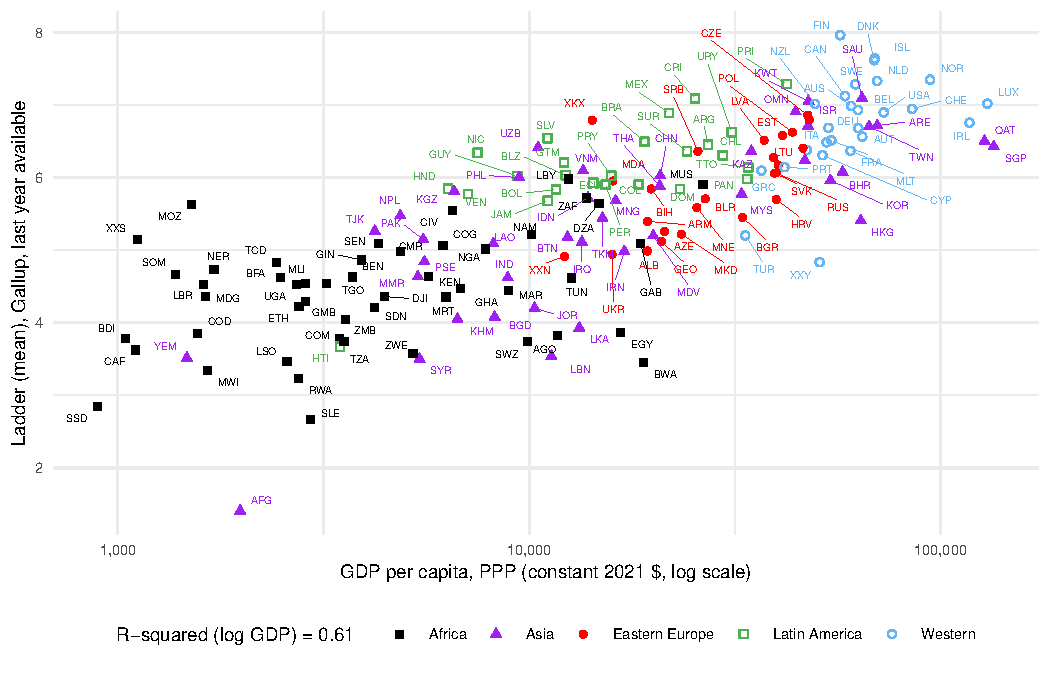
\includegraphics[width=.95\textwidth]{../figures/main/gallup_ladder_mean_vs_gdp_ppp.pdf}
\end{figure}

\begin{table}[htbp]
    \centering
    \caption{Share of explained variance due to income rather than region (LMG), Gallup, last observation per country.}\label{tab:share_gallup}
    \begin{adjustbox}{max width=\textwidth}
    \begin{tabular}{lccccccc}
\toprule
Well-being indicator & \multicolumn{2}{c}{log GDP p.c.} & Sextile & \multicolumn{4}{c}{Income cluster} \\ & PPP & nominal & PPP & $k$=5 PPP & $k$=6 PPP & $k$=7 PPP & $k$=7 nominal \\
\midrule
Satisfied & \textbf{0.58} & \textbf{0.61} & \textbf{0.59} & \textbf{0.58} & \textbf{0.60} & \textbf{0.59} & \textbf{0.60} \\
Very satisfied (8--10) & 0.44 & \textbf{0.51} & 0.49 & 0.47 & 0.49 & \textbf{0.51} & \textbf{0.53} \\
Extremely satisfied (9--10) & 0.16 & 0.25 & 0.24 & 0.27 & 0.22 & 0.30 & 0.28 \\
Completely satisfied (10) & 0.02 & 0.02 & 0.08 & 0.09 & 0.06 & 0.08 & 0.08 \\
Unsatisfied (0/1--4) & \textbf{0.61} & \textbf{0.60} & \textbf{0.60} & \textbf{0.59} & \textbf{0.61} & \textbf{0.60} & \textbf{0.59} \\
Dissatisfied (0/1--2) & \textbf{0.66} & \textbf{0.63} & \textbf{0.67} & \textbf{0.66} & \textbf{0.67} & \textbf{0.67} & \textbf{0.65} \\
Satisfaction (mean) & \textbf{0.60} & \textbf{0.62} & \textbf{0.59} & \textbf{0.58} & \textbf{0.60} & \textbf{0.59} & \textbf{0.60} \\
\midrule
Mean & 0.44 & 0.46 & 0.47 & 0.46 & 0.47 & 0.48 & 0.48 \\
Max & 0.66 & 0.63 & 0.67 & 0.66 & 0.67 & 0.67 & 0.65 \\
\bottomrule
\end{tabular}

    \end{adjustbox}
    \begin{minipage}{\textwidth}\footnotesize \textit{Note:} \nGallupCountries countries, last Gallup observation available (2006--2023). Same definitions as Table~\ref{tab:share_income}. Values above 0.5 (income is the better predictor) are in bold.\end{minipage}
\end{table}

\subsection{Other correlates, within-country evidence and happiest countries}\label{subsec:correlates}

What do regions capture? The average perceived freedom of choice and control over one's life alone explains \RtwoFreedomSatisfaction\% of the variance of mean satisfaction; in a Shapley decomposition with income and region, it accounts for \shapleyFreedom percentage points, against \shapleyFreedomRegion for region and \shapleyFreedomIncome for income (Appendix Table~\ref{tab:correlates}). This variable is itself a subjective evaluation, so the correlation should not be read causally, but it suggests that non-material dimensions of life are central to regional differences \citep{inglehart_development_2008}. Tolerance of homosexuality (\RtwoTolerance\%), the importance of God (\RtwoGod\%) and GDP growth over the previous five years (\RtwoGrowth\%) explain much less.

The cross-sectional relation should not be confused with the relation over time. Within countries (country fixed effects, \nWithin observations), mean satisfaction increases with log GDP per capita, with a slope of \withinSlopeSatisfiedMean per unit of $\log_{10}$ GDP, larger than the cross-sectional slope (\crossSlopeSatisfiedMean), although income growth explains only \withinRtwoSatisfiedMean of the within-country variance (Appendix Table~\ref{tab:within}). These associations are consistent with \citet{stevenson_economic_2008} and \citet{sacks_new_2012} rather than with a strict version of the Easterlin paradox \citep{easterlin_does_1974,easterlin_happiness_2010}, although they may reflect common shocks (e.g.\ transition recessions) rather than the effect of income per se.

Finally, rankings of countries depend on the indicator. Counting, for each indicator and each wave (and all waves combined), the happiest country-year, \happiestFirst appears most often (\happiestFirstN times out of \nHappiestCells), followed by \happiestSecond (\happiestSecondN) and \happiestThird (\happiestThirdN) (Appendix Table~\ref{tab:happiest}). The happiest country-years are Western (\happiestRegionWestern), Latin American (\happiestRegionLatinAmerica), Asian (\happiestRegionAsia) or African (\happiestRegionAfrica). Similarly, with Gallup data on emotions, \citet{blanchflower_wellbeing_2024} find that the top-ranked country or U.S.\ state differs across measures: Denmark for the ladder, Hawaii for enjoyment, Paraguay for smiling, Bhutan for being well-rested, and Vietnam, Taiwan, Uzbekistan and Finland for the lowest prevalence of pain, sadness, worry and anger, respectively. The link between income and well-being seems to be that rich countries rarely experience low well-being, rather than that they reach the highest levels.


\section{Discussion}\label{sec:discussion}
% Shared section: interpretation and limitations of the region vs. income analysis
Region is not a mechanism: it bundles culture, history, institutions, social ties, and possibly cross-cultural differences in how people use response scales \citep{chen_response_1995,diener_personality_2003,exton_comparing_2015}. If regional differences partly reflect response styles, region predicts \textit{measured} rather than \textit{experienced} well-being. Studies of migrants suggest that national differences partly reflect a cultural determinant of well-being rather than translation artifacts \citep{senik_french_2014,exton_comparing_2015}, but the present analysis cannot separate these interpretations; anchoring vignettes \citep{kapteyn_life_2010} or measures of emotional well-being would help. Moreover, the advantage of region rests on Latin America and Eastern Europe. The fairest summary is that GDP per capita leaves much of the cross-country variation unexplained, and that a few large regional deviations explain more of it than income does in the WVS.

The modest cross-country role of income echoes within-country evidence. Studies comparing people within countries find a small effect of income on life satisfaction relative to other circumstances such as employment or marital status \citep{helliwell_hows_2003,blanchflower_well-being_2004}; \citet{kahneman_would_2006} argue that even these estimates overstate the role of income, because of a ``focusing illusion'' when people evaluate their lives; and in German panel data, life satisfaction adapts to income increases within a few years \citep{di_tella_happiness_2010}. Conversely, emotional well-being increases with log income for most people in the United States \citep{killingsworth_income_2023}, and the within-country association between GDP and satisfaction documented above shows that the weak cross-sectional relation does not imply that income is irrelevant.


The main qualification is that the WVS and Gallup disagree on the strength of the relation between income and well-being. WVS samples are less representative in poorer countries, as noted by \citet{deaton_income_2008}: they over-represent tertiary-educated adults by a median factor of \ratioTertiaryLow in countries below 10,000 dollars of GDP per capita, against \ratioTertiaryHigh above 30,000 dollars. Yet reweighting WVS samples to the population share of tertiary-educated adults barely changes their relation with income ($R^2$ from \RtwoCommonWVSraw to \RtwoCommonWVSeduAdj, against \RtwoCommonGallupSub for Gallup). The companion paper \todo{cite} investigates this discrepancy with a survey experiment in ten high-income countries: asked to the same sample, the ladder is better predicted by GDP than the satisfaction question, which reproduces about half of the Gallup--WVS difference in $R^2$, but both questions yield an income gradient close to Gallup's. In the absence of evidence on which dataset better measures national well-being in low-income countries, where the two disagree most, conclusions about the global income--well-being relationship should be reported for both.

\section{Conclusion}\label{sec:conclusion}

GDP per capita is a weaker predictor of national well-being than is often assumed, but how weak depends on the data. In the WVS, it explains a small share of the cross-country variance of well-being, less than a country's world region, and essentially nothing of the share of very happy people. The richest countries are not necessarily the happiest: the country-year with the highest share of very happy people in the WVS is Kyrgyzstan in 2020 (\veryHappyKGZ\%, with a mean life satisfaction of \satisfactionKGZ), with a GDP per capita of about \gdpKGZ dollars; and many middle-income countries, especially in Latin America, are as satisfied as the richest ones. In the Gallup World Poll, however, income predicts life evaluations as well as region, and within countries well-being rises with GDP over time.

These results suggest that absolute income is less determining for national well-being than the cross-country correlations often cited imply: rich countries rarely have low well-being, but growth is neither necessary nor sufficient for high well-being. Well-being itself, rather than growth, its imprecise proxy, should be the primary target when evaluating reforms. Non-material dimensions associated with regions---social ties, perceived freedom, history, culture---deserve more attention, both in research on the mechanisms behind regional differences and in policy evaluation \citep{stiglitz_report_2009,frijters_happy_2020}. Future research should test whether emotions are also better predicted by region than by income \citep{blanchflower_wellbeing_2024,killingsworth_income_2023}, and, despite evidence against translation issues \citep{diener_culture_2000}, use anchoring vignettes to separate true differences in well-being from differences in response styles.

\section*{Declaration of generative AI and AI-assisted technologies in the writing process}
During the preparation of this work the author used Claude Opus 5.5 to write analysis code and draft parts of the manuscript. After using this tool, the author reviewed and edited the code and content created by AI as needed and takes full responsibility for the content of the publication.

\bibliography{wellbeing}

\clearpage
\appendix
\section{Additional results}\label{app:additional}
\renewcommand{\thetable}{A\arabic{table}}
\renewcommand{\thefigure}{A\arabic{figure}}
\setcounter{table}{0}
\setcounter{figure}{0}

\begin{table}[htbp]
    \centering
    \caption{Correlation between national well-being indicators (WVS country-years).}\label{tab:correlation}
    \begin{adjustbox}{max width=\textwidth}
    \begin{tabular}{lcccccccc}
\toprule
& Happy & Very Happy & Very Unhappy & V. Happy -- V. Unhappy & Happiness (mean) & Satisfaction (mean) & Satisfied & Happy + Satisfied \\
\midrule
Happy & 1.00 & 0.61 & -0.73 & 0.70 & 0.90 & 0.72 & 0.72 & 0.90 \\
Very Happy & 0.61 & 1.00 & -0.38 & 0.98 & 0.89 & 0.63 & 0.53 & 0.61 \\
Very Unhappy & -0.73 & -0.38 & 1.00 & -0.55 & -0.68 & -0.57 & -0.57 & -0.68 \\
V. Happy -- V. Unhappy & 0.70 & 0.98 & -0.55 & 1.00 & 0.95 & 0.69 & 0.60 & 0.69 \\
Happiness (mean) & 0.90 & 0.89 & -0.68 & 0.95 & 1.00 & 0.76 & 0.70 & 0.84 \\
Satisfaction (mean) & 0.72 & 0.63 & -0.57 & 0.69 & 0.76 & 1.00 & 0.96 & 0.93 \\
Satisfied & 0.72 & 0.53 & -0.57 & 0.60 & 0.70 & 0.96 & 1.00 & 0.95 \\
Happy + Satisfied & 0.90 & 0.61 & -0.68 & 0.69 & 0.84 & 0.93 & 0.95 & 1.00 \\
\bottomrule
\end{tabular}

    \end{adjustbox}
    \begin{minipage}{\textwidth}\footnotesize \hfill(Back~to~Section~\ref{subsec:wvs}.)\end{minipage}
\end{table}

\begin{table}[htbp]
    \centering
    \caption{Slope of national well-being indicators with respect to $\log_{10}$ GDP per capita (PPP).}\label{tab:slopes}
    \begin{adjustbox}{max width=\textwidth}
    \begin{tabular}{llccccc}
\toprule
Data & Indicator & Slope & s.e. & $p$-value & $R^2$ & Obs. \\
\midrule
WVS & Happy & 0.109 & 0.019 & 0.000 & 0.145 & 337 \\
WVS & Very Happy & 0.003 & 0.025 & 0.915 & 0.000 & 337 \\
WVS & Very Unhappy & \ensuremath{-}0.022 & 0.004 & 0.000 & 0.072 & 337 \\
WVS & V. Happy -- V. Unhappy & 0.024 & 0.026 & 0.356 & 0.004 & 337 \\
WVS & Happiness (mean) & 0.268 & 0.083 & 0.001 & 0.045 & 337 \\
WVS & Satisfaction (mean) & 1.144 & 0.142 & 0.000 & 0.234 & 337 \\
WVS & Satisfied & 0.237 & 0.024 & 0.000 & 0.317 & 337 \\
WVS & Happy + Satisfied & 0.173 & 0.019 & 0.000 & 0.276 & 335 \\
\midrule
Gallup & Satisfied & 0.372 & 0.017 & 0.000 & 0.655 & 2344 \\
Gallup & Very satisfied (8--10) & 0.218 & 0.018 & 0.000 & 0.442 & 2344 \\
Gallup & Extremely satisfied (9--10) & 0.065 & 0.009 & 0.000 & 0.178 & 2344 \\
Gallup & Completely satisfied (10) & 0.012 & 0.005 & 0.008 & 0.015 & 2344 \\
Gallup & Unsatisfied (0/1--4) & \ensuremath{-}0.304 & 0.012 & 0.000 & 0.639 & 2344 \\
Gallup & Dissatisfied (0/1--2) & \ensuremath{-}0.135 & 0.009 & 0.000 & 0.432 & 2344 \\
Gallup & Satisfaction (mean) & 1.779 & 0.083 & 0.000 & 0.611 & 2344 \\
\bottomrule
\end{tabular}

    \end{adjustbox}
    \begin{minipage}{\textwidth}\footnotesize \textit{Note:} OLS across country-years; standard errors clustered by country. Gallup: 2006--2023. \hfill(Back~to~Section~\ref{subsec:r2_income}.)\end{minipage}
\end{table}

\begin{table}[htbp]
    \centering
    \caption{Out-of-sample predictive capacity: leave-one-country-out cross-validated $R^2$.}\label{tab:cv}
    \begin{adjustbox}{max width=\textwidth}
    \begin{tabular}{llccccc}
\toprule
Data & Indicator & Obs. & log GDP PPP & Best income variable & Region & log GDP PPP + Region \\
\midrule
WVS, all waves & Happy & 302 & 0.11 & 0.17 & 0.31 & 0.36 \\
WVS, all waves & Very Happy & 302 & -0.03 & -0.06 & 0.29 & 0.29 \\
WVS, all waves & Very Unhappy & 302 & 0.05 & 0.09 & 0.11 & 0.12 \\
WVS, all waves & V. Happy -- V. Unhappy & 302 & -0.02 & -0.05 & 0.30 & 0.29 \\
WVS, all waves & Happiness (mean) & 302 & 0.02 & 0.03 & 0.33 & 0.33 \\
WVS, all waves & Satisfaction (mean) & 302 & 0.18 & 0.19 & 0.44 & 0.51 \\
WVS, all waves & Satisfied & 302 & 0.26 & 0.30 & 0.42 & 0.53 \\
WVS, all waves & Happy + Satisfied & 300 & 0.23 & 0.28 & 0.42 & 0.51 \\
\midrule
WVS, last obs. per country & Happy & 108 & 0.05 & 0.10 & 0.24 & 0.26 \\
WVS, last obs. per country & Very Happy & 108 & -0.01 & -0.04 & 0.25 & 0.24 \\
WVS, last obs. per country & Very Unhappy & 108 & 0.04 & 0.04 & 0.05 & 0.07 \\
WVS, last obs. per country & V. Happy -- V. Unhappy & 108 & -0.02 & -0.06 & 0.25 & 0.24 \\
WVS, last obs. per country & Happiness (mean) & 108 & -0.04 & -0.04 & 0.26 & 0.24 \\
WVS, last obs. per country & Satisfaction (mean) & 108 & 0.13 & 0.12 & 0.36 & 0.40 \\
WVS, last obs. per country & Satisfied & 108 & 0.22 & 0.23 & 0.34 & 0.42 \\
WVS, last obs. per country & Happy + Satisfied & 108 & 0.18 & 0.20 & 0.36 & 0.42 \\
\midrule
Gallup, all years (2006--23) & Satisfaction (mean) & 2344 & 0.61 & 0.66 & 0.49 & 0.68 \\
Gallup, all years (2006--23) & Satisfied & 2344 & 0.65 & 0.72 & 0.52 & 0.72 \\
Gallup, all years (2006--23) & Unsatisfied (0/1--4) & 2344 & 0.63 & 0.65 & 0.48 & 0.68 \\
\midrule
Gallup, last obs. per country & Satisfaction (mean) & 167 & 0.60 & 0.58 & 0.45 & 0.64 \\
Gallup, last obs. per country & Satisfied & 167 & 0.65 & 0.68 & 0.52 & 0.70 \\
Gallup, last obs. per country & Unsatisfied (0/1--4) & 167 & 0.65 & 0.60 & 0.48 & 0.67 \\
\midrule
WHR, 2023--25 average & Satisfaction (mean) & 147 & 0.62 & 0.60 & 0.52 & 0.69 \\
\bottomrule
\end{tabular}

    \end{adjustbox}
    \begin{minipage}{\textwidth}\footnotesize \textit{Note:} Each country's observations are predicted with a model estimated on all other countries. Cross-validated $R^2 = 1 - \sum (y - \hat y_{\text{out-of-sample}})^2 / \sum (y - \bar y)^2$; it can be negative when a model predicts worse than the overall mean. In each row, the highest cross-validated $R^2$ among log GDP PPP, the best income variable and region is in bold. \hfill(Back~to~Section~\ref{subsec:region_wvs}.)\end{minipage}
\end{table}

\begin{table}[htbp]
    \centering
    \caption{Robustness: income vs.\ region across specifications and datasets.}\label{tab:robustness}
    \begin{adjustbox}{max width=\textwidth}
    \begin{tabular}{lccccccccc}
\toprule
Specification & Obs. & Countries & \multicolumn{2}{c}{$R^2$ income} & $R^2$ region & \multicolumn{3}{c}{Share of explained variance due to income} & Region better \\ & & & log PPP & best & & log PPP & best & adj. $R^2$ & (share of cases) \\
\midrule
WVS, all waves & 302 & 108 & 0.12 & 0.19 & 0.37 & 0.18 & 0.28 & 0.22 & 1.00 \\
WVS, waves 1--2 (1981--91) & 26 & 21 & 0.07 & 0.43 & 0.58 & 0.09 & 0.40 & 0.10 & 1.00 \\
WVS, wave 3 (1995--99) & 55 & 55 & 0.16 & 0.33 & 0.65 & 0.14 & 0.28 & 0.18 & 1.00 \\
WVS, wave 4 (1999--2004) & 40 & 40 & 0.19 & 0.31 & 0.33 & 0.27 & 0.47 & 0.47 & 0.43 \\
WVS, wave 5 (2004--09) & 58 & 58 & 0.21 & 0.35 & 0.49 & 0.22 & 0.38 & 0.23 & 0.98 \\
WVS, wave 6 (2010--16) & 60 & 60 & 0.08 & 0.22 & 0.27 & 0.14 & 0.41 & 0.19 & 0.96 \\
WVS, wave 7 (2017--22) & 64 & 64 & 0.07 & 0.13 & 0.26 & 0.20 & 0.31 & 0.14 & 1.00 \\
WVS, wave 7 w/o 2020--21 & 45 & 45 & 0.06 & 0.22 & 0.31 & 0.14 & 0.41 & 0.14 & 0.95 \\
WVS, population-weighted & 302 & 108 & 0.10 & 0.19 & 0.23 & 0.24 & 0.44 & 0.33 & 0.84 \\
WVS, last obs. per country & 108 & 108 & 0.10 & 0.18 & 0.33 & 0.18 & 0.32 & 0.21 & 0.96 \\
WVS, no GDP imputation & 283 & 104 & 0.12 & 0.19 & 0.38 & 0.17 & 0.28 & 0.21 & 1.00 \\
WVS, GDP PPP 2017 \$ (old) & 302 & 108 & 0.13 & 0.19 & 0.37 & 0.19 & 0.28 & 0.22 & 1.00 \\
WVS, w/o Latin Am. \& E. Europe & 185 & 68 & 0.16 & 0.27 & 0.18 & 0.34 & 0.68 & 0.54 & 0.27 \\
WVS, 6 regions & 302 & 108 & 0.12 & 0.19 & 0.35 & 0.18 & 0.28 & 0.22 & 1.00 \\
WVS, World Bank regions (7) & 302 & 108 & 0.12 & 0.19 & 0.22 & 0.31 & 0.43 & 0.38 & 0.64 \\
WVS, continents (5) & 302 & 108 & 0.12 & 0.19 & 0.20 & 0.34 & 0.46 & 0.41 & 0.54 \\
WVS, UN sub-regions & 302 & 108 & 0.12 & 0.19 & 0.40 & 0.20 & 0.29 & 0.25 & 1.00 \\
\midrule
Gallup, all years (2006--23) & 2344 & 167 & 0.42 & 0.48 & 0.42 & 0.46 & 0.51 & 0.49 & 0.31 \\
Gallup, last obs. per country & 167 & 167 & 0.42 & 0.44 & 0.41 & 0.44 & 0.48 & 0.45 & 0.37 \\
Gallup, last obs., WVS countries & 105 & 105 & 0.43 & 0.46 & 0.42 & 0.46 & 0.49 & 0.47 & 0.37 \\
Gallup, last obs., 6 regions & 167 & 167 & 0.42 & 0.44 & 0.42 & 0.43 & 0.46 & 0.44 & 0.41 \\
Gallup, last obs., WB regions & 167 & 167 & 0.42 & 0.44 & 0.38 & 0.47 & 0.50 & 0.48 & 0.29 \\
WHR, 2023--25 average & 147 & 147 & 0.63 & 0.63 & 0.55 & 0.56 & 0.56 & 0.56 & 0.00 \\
\bottomrule
\end{tabular}

    \end{adjustbox}
    \begin{minipage}{\textwidth}\footnotesize \textit{Note:} Averages over well-being indicators (8 for the WVS; 7 satisfaction indicators for Gallup; mean ladder for the WHR). ``Best'' refers to the income measure with the highest average $R^2$ in the main WVS specification (\bestIncome). ``Region better'' is the share of indicator $\times$ income-measure combinations for which $s < 0.5$; values above 0.5 are in bold. Alternative region classifications and exclusions of regions: see Table~\ref{tab:region_classifications}. \hfill(Back~to~Section~\ref{subsec:region_wvs}.)\end{minipage}
\end{table}

\begin{table}[htbp]
    \centering
    \caption{Other country-level correlates of national well-being: Shapley decomposition of $R^2$ (WVS).}\label{tab:correlates}
    \begin{adjustbox}{max width=\textwidth}
    \begin{tabular}{llcccccc}
\toprule
Indicator & Other variable & Obs. & $R^2$ other alone & \multicolumn{4}{c}{Shapley decomposition of $R^2$} \\ & & & & Income & Region & Other & Total \\
\midrule
Satisfaction (mean) & Freedom of choice & 334 & 0.63 & 0.11 & 0.21 & \textbf{0.42} & 0.74 \\
Satisfaction (mean) & Importance of God & 329 & 0.01 & 0.17 & \textbf{0.33} & 0.02 & 0.51 \\
Satisfaction (mean) & Tolerance (homosexuality) & 326 & 0.24 & 0.12 & \textbf{0.30} & 0.10 & 0.52 \\
Satisfaction (mean) & Importance of democracy & 216 & 0.08 & 0.13 & \textbf{0.32} & 0.02 & 0.47 \\
Satisfaction (mean) & GDP growth (5-year) & 334 & 0.02 & 0.16 & \textbf{0.34} & 0.02 & 0.52 \\
\midrule
Happiness (mean) & Freedom of choice & 333 & 0.39 & 0.02 & 0.22 & \textbf{0.27} & 0.51 \\
Happiness (mean) & Importance of God & 330 & 0.01 & 0.05 & \textbf{0.31} & 0.03 & 0.39 \\
Happiness (mean) & Tolerance (homosexuality) & 325 & 0.09 & 0.02 & \textbf{0.31} & 0.07 & 0.40 \\
Happiness (mean) & Importance of democracy & 216 & 0.03 & 0.02 & \textbf{0.28} & \ensuremath{-}0.03 & 0.27 \\
Happiness (mean) & GDP growth (5-year) & 334 & 0.01 & 0.03 & \textbf{0.31} & 0.00 & 0.34 \\
\bottomrule
\end{tabular}

    \end{adjustbox}
    \begin{minipage}{\textwidth}\footnotesize \textit{Note:} Country-year averages of WVS variables: perceived freedom of choice and control (1--10), importance of God in one's life (1--10), justifiability of homosexuality (1--10), importance of living in a democracy (1--10, waves 5--7), and average annual growth of real GDP per capita over the previous five years. Shapley decomposition of the $R^2$ of the regression on log GDP per capita, region dummies and the other variable. In each row, the largest contribution among income, region and the other variable is in bold. \hfill(Back~to~Section~\ref{subsec:correlates}.)\end{minipage}
\end{table}

\begin{table}[htbp]
    \centering
    \caption{Within-country relation between national well-being and $\log_{10}$ GDP per capita (country fixed effects, WVS).}\label{tab:within}
    \begin{adjustbox}{max width=\textwidth}
    \begin{tabular}{lccccc}
\toprule
Indicator & Slope & s.e. & $p$-value & Within $R^2$ & Obs. \\
\midrule
Happy & 0.281 & 0.042 & 0.000 & 0.276 & 309 \\
Very Happy & 0.204 & 0.048 & 0.000 & 0.142 & 309 \\
Very Unhappy & \ensuremath{-}0.038 & 0.009 & 0.000 & 0.042 & 309 \\
V. Happy -- V. Unhappy & 0.242 & 0.054 & 0.000 & 0.156 & 309 \\
Happiness (mean) & 1.046 & 0.178 & 0.000 & 0.240 & 309 \\
Satisfaction (mean) & 2.275 & 0.412 & 0.000 & 0.340 & 309 \\
Satisfied & 0.434 & 0.075 & 0.000 & 0.343 & 309 \\
Happy + Satisfied & 0.361 & 0.057 & 0.000 & 0.386 & 307 \\
\bottomrule
\end{tabular}

    \end{adjustbox}
    \begin{minipage}{\textwidth}\footnotesize \textit{Note:} Countries surveyed at least twice. Standard errors clustered by country. On average over the eight indicators, the within-country $R^2$ is \meanWithinRtwo. \hfill(Back~to~Section~\ref{subsec:correlates}.)\end{minipage}
\end{table}

\begin{table}[htbp]
    \centering
    \caption{Countries most often ranked happiest (WVS, 8 indicators $\times$ 8 samples: each wave and all waves combined).}\label{tab:happiest}
    \begin{tabular}{lcl}
\toprule
Country & Occurrences as happiest & Region \\
\midrule
Switzerland & 10 & Western \\
Mexico & 9 & Latin America \\
Kyrgyzstan & 6 & Asia \\
Australia & 5 & Western \\
Nigeria & 4 & Africa \\
Puerto Rico & 4 & Latin America \\
Vietnam & 4 & Asia \\
Colombia & 3 & Latin America \\
Finland & 3 & Western \\
Netherlands & 3 & Western \\
\bottomrule
\end{tabular}

    \begin{minipage}{\textwidth}\footnotesize \textit{Note:} Looking at all waves combined, the happiest country-year is: \happiestAllWaves. For \textit{Very Unhappy}, the happiest country-year is the one with the lowest share. \hfill(Back~to~Section~\ref{subsec:correlates}.)\end{minipage}
\end{table}

\begin{figure}[htbp]
    \centering
    \caption{Share of \textit{Very happy} people vs.\ GDP per capita (PPP), WVS/EVS 1981--2023.}\label{fig:very_happy_gdp}
    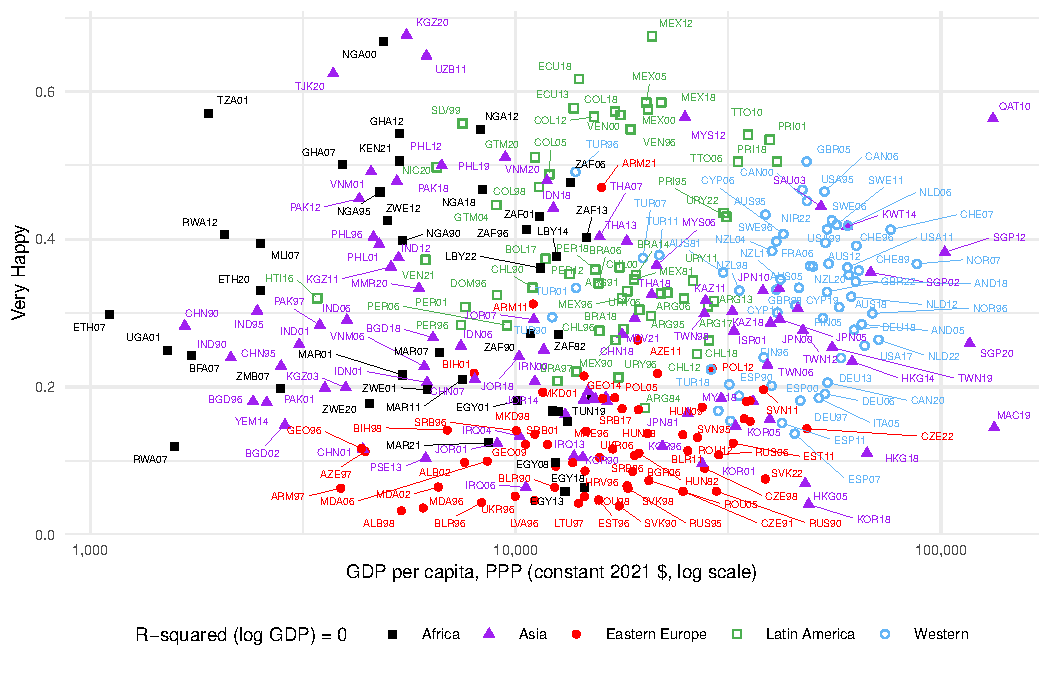
\includegraphics[width=.9\textwidth]{../figures/main/wvs_very_happy_vs_gdp_ppp.pdf}
\end{figure}

\begin{figure}[htbp]
    \centering
    \caption{\textit{Happy} vs.\ GDP per capita (PPP), WVS/EVS 1981--2023.}\label{fig:happy_gdp}
    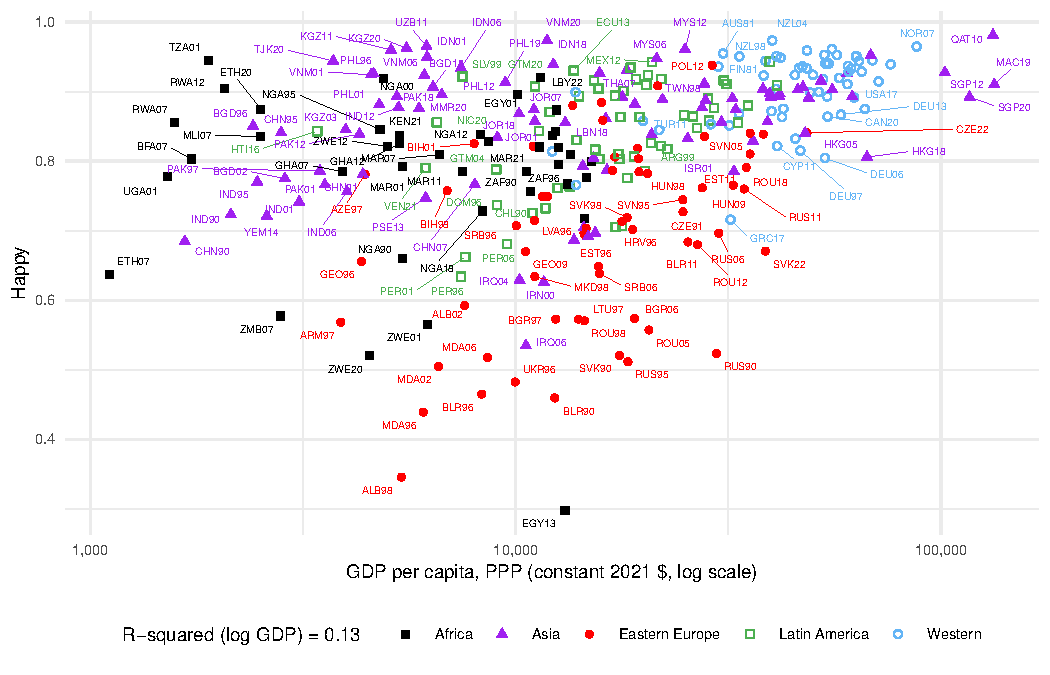
\includegraphics[width=.9\textwidth]{../figures/main/wvs_happy_vs_gdp_ppp.pdf}
\end{figure}

\begin{figure}[htbp]
    \centering
    \caption{\textit{Very Unhappy} vs.\ GDP per capita (PPP), WVS/EVS 1981--2023.}\label{fig:very_unhappy_gdp}
    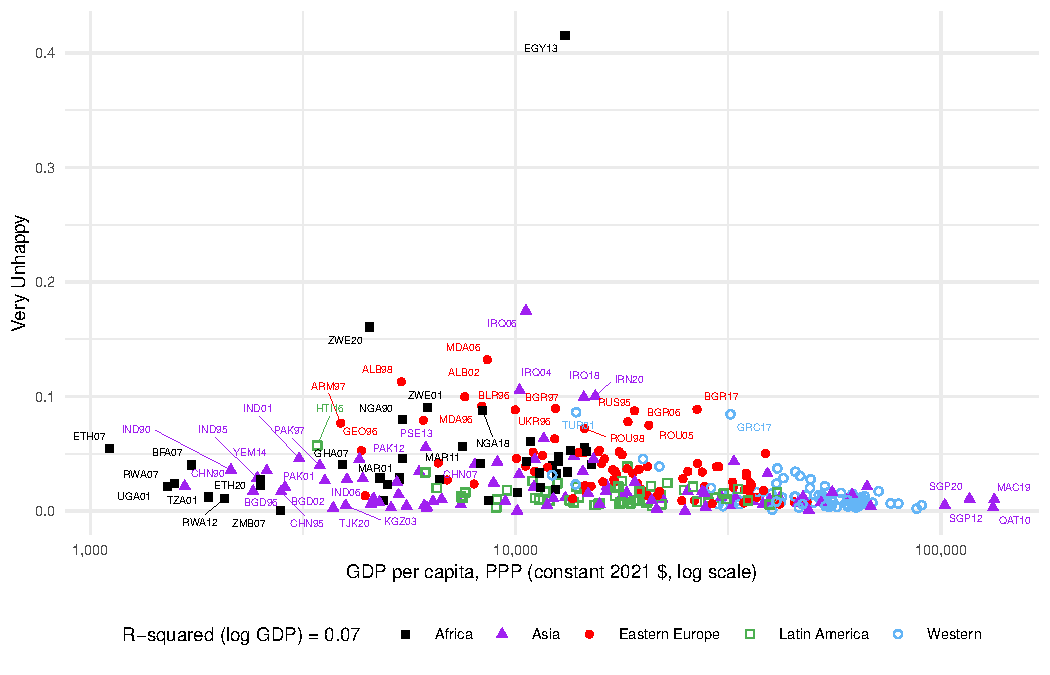
\includegraphics[width=.9\textwidth]{../figures/main/wvs_very_unhappy_vs_gdp_ppp.pdf}
    \begin{minipage}{.9\textwidth}\footnotesize \textit{Note:} Egypt 2013 (\veryUnhappyEGY\% of very unhappy people) is not shown, to keep the $y$-axis readable; the $R^2$ in the legend includes it.\end{minipage}
\end{figure}

\begin{figure}[htbp]
    \centering
    \caption{\textit{V.~Happy -- V.~Unhappy} vs.\ GDP per capita (PPP), WVS/EVS 1981--2023.}\label{fig:vhmvu_gdp}
    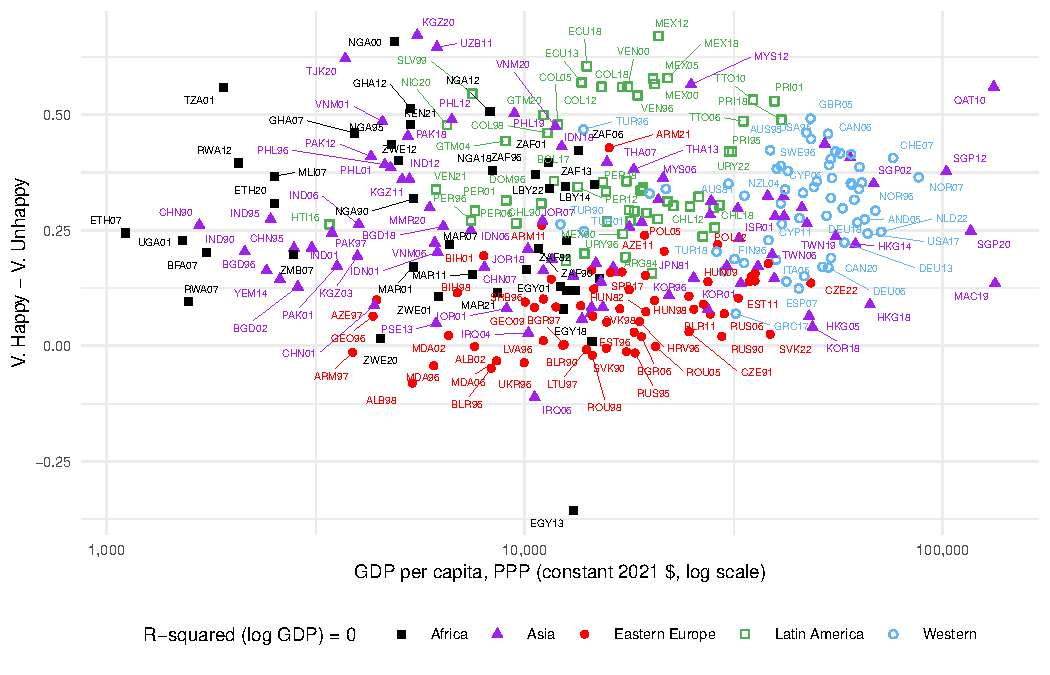
\includegraphics[width=.9\textwidth]{../figures/main/wvs_very_happy_minus_very_unhappy_vs_gdp_ppp.pdf}
\end{figure}

\begin{figure}[htbp]
    \centering
    \caption{\textit{Satisfied} vs.\ GDP per capita (PPP), WVS/EVS 1981--2023.}\label{fig:satisfied_gdp}
    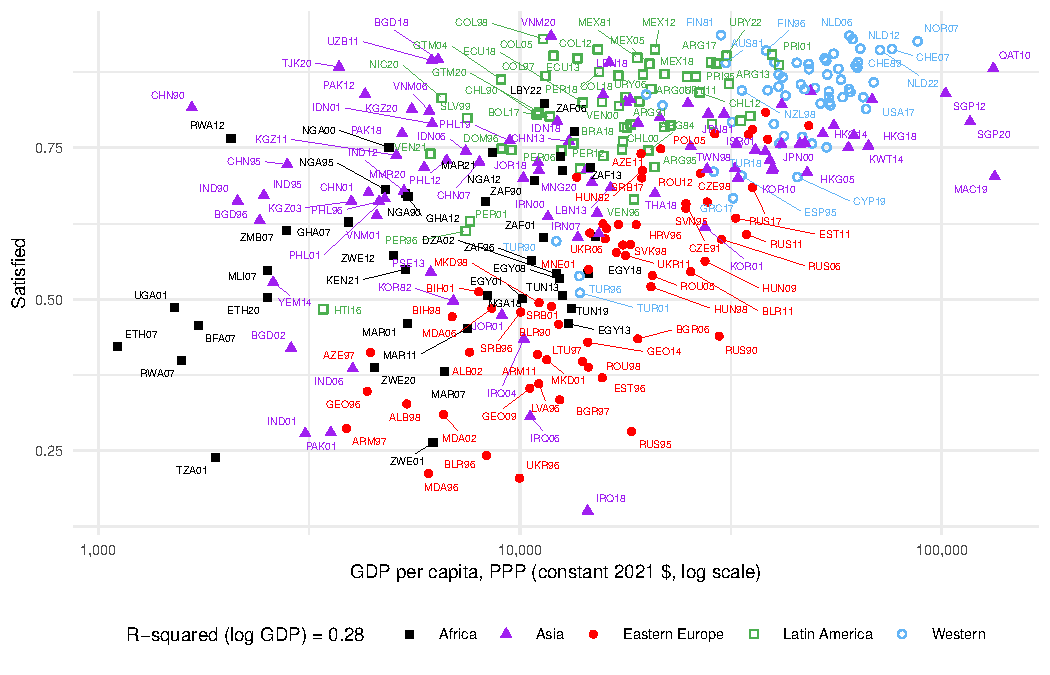
\includegraphics[width=.9\textwidth]{../figures/main/wvs_satisfied_vs_gdp_ppp.pdf}
\end{figure}

\begin{figure}[htbp]
    \centering
    \caption{\textit{Happy + Satisfied} vs.\ GDP per capita (PPP), WVS/EVS 1981--2023.}\label{fig:layard_gdp}
    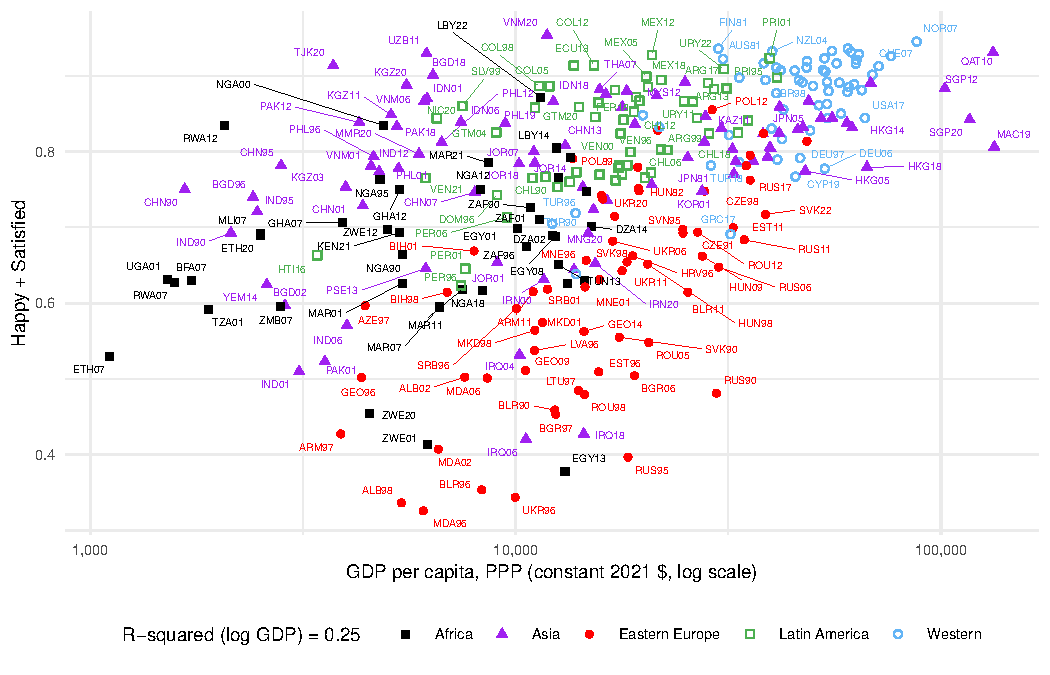
\includegraphics[width=.9\textwidth]{../figures/main/wvs_happiness_layard_vs_gdp_ppp.pdf}
\end{figure}

\begin{figure}[htbp]
    \centering
    \caption{\textit{Happy} vs.\ GDP per capita (nominal), WVS/EVS wave 7 (2017--2023), weighted by population.}\label{fig:happy_gdp_w7_weighted}
    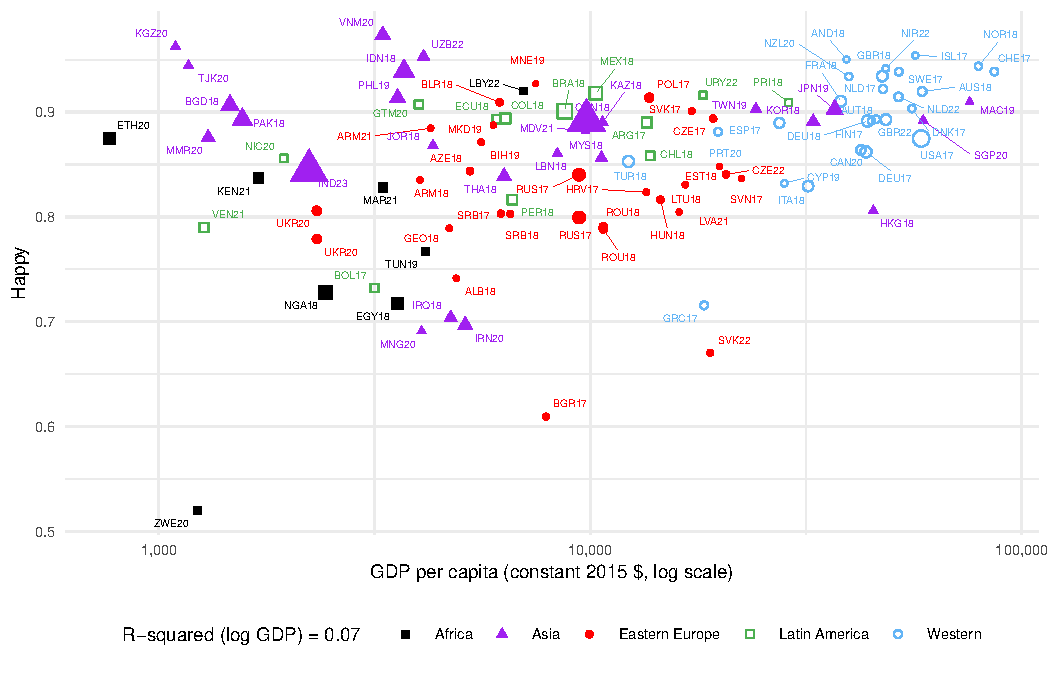
\includegraphics[width=.9\textwidth]{../figures/main/wvs_happy_vs_gdp_wave7_weighted.pdf}
    \begin{minipage}{.9\textwidth}\footnotesize \textit{Note:} Point size and regression weights proportional to population. \hfill(Back~to~Section~\ref{subsec:r2_income}.)\end{minipage}
\end{figure}

\end{document}
